\section{Lines}

\subsection{Definition: \texttt{\textbackslash tkzDefLine}}

\subsubsection{Mediator}

\begin{tkzexample}[latex=5cm,small]
  \begin{tikzpicture}[scale=0.7]
    \tkzSetUpPoint[size=1.5pt]
    \tkzDefPoints{-2/0/A,1/2/B}
    \tkzDefLine[mediator](A,B)
    \tkzGetPoints{C}{D}
    \tkzInterLL(C,D)(A,B)
    \tkzGetPoint{I}
    \tkzDrawPoints(A,B)
    \tkzDrawSegments(A,B C,D)
    \tkzMarkRightAngle[size=.2](A,I,C)
    \tkzMarkSegments[mark=||](A,I B,I)
  \end{tikzpicture}
\end{tkzexample}

\subsubsection{Bisector}

\begin{tkzexample}[latex=5cm,small]
  \begin{tikzpicture}[rotate=25,scale=.7]
    \tkzDefPoints{0/0/C, 2/-3/A, 4/0/B}
    \tkzDefLine[bisector,K=.5](B,A,C)
    \tkzGetPoint{a}
    \tkzDrawLines[add= 0 and .5](A,B A,C)
    \tkzShowLine[bisector,gap=4,size=2,color=red](B,A,C)
    \tkzDrawLines[blue!50,dashed,add= 0 and .5](A,a)
    \tkzLabelPoints[below](A,C)
    \tkzLabelPoints[right](B)
    \tkzDrawPoints[size=1.5pt](A,B,C,a)
  \end{tikzpicture}
\end{tkzexample}

\subsubsection{Orthogonal And Parallel}

\begin{tkzexample}[latex=5cm,small]
  \begin{tikzpicture}
    \tkzDefPoints{-1.5/-0.25/A,1/-0.75/B,-0.7/1/C}
    \tkzDrawLine(A,B)
    \tkzDefLine[orthogonal=through C](B,A)
    \tkzGetPoint{c}    \tkzDrawLine(C,c)
    \tkzInterLL(A,B)(C,c)    \tkzGetPoint{I}
    \tkzDefLine[parallel=through C](A,B)
    \tkzGetPoint{D}    \tkzDrawLine(C,D)
    \tkzDrawPoints(A,B,C,c,D)
    \tkzLabelPoints[above right](A,B,C,c,D)
    \tkzLabelLine[pos=1.25,below left](A,B){$(l_1)$}
    \tkzLabelLine[pos=1.2,right](C,D){$(l_2)$}
    \tkzLabelLine[pos=1.25,left](C,c){$\delta$}
    \tkzMarkRightAngle(C,I,B)\tkzMarkRightAngle(I,C,D)
  \end{tikzpicture}
\end{tkzexample}

\subsection{Tangent to a Circle: \texttt{\textbackslash tkzDefTangent}}

\begin{tkzexample}[latex=5cm,small]
  \begin{tikzpicture}[scale=.75]
    \tkzDefPoint(0,0){O}
    \tkzDefRandPointOn[circle=center O radius 2]
    \tkzGetPoint{A}
    \tkzDrawSegment(O,A)
    \tkzDrawCircle(O,A)
    \tkzDefTangent[at=A](O)    \tkzGetPoint{h}
    \tkzDrawPoints[size=1.5pt](A,O,h)
    \tkzDrawLine[add = 2 and 2.5](A,h)
    \tkzMarkRightAngle[fill=red!30](O,A,h)
    \tkzLabelPoints[above right](A) \tkzLabelPoints[left](O)
  \end{tikzpicture}
\end{tkzexample}

\subsection{Median, Altitude, and Bisector}

\begin{tkzexample}[latex=5cm,small]
  \begin{tikzpicture}[scale=1.2]
    \tkzDefPoint(0,0){A}
    \tkzDefPoint(4,0){B}
    \tkzDefPoint(1,3){C}
    \tkzDrawPolygon[densely dashed](A,B,C)
    \tkzSetUpLine[color=blue]
    \tkzDefSpcTriangle[medial,name=M](A,B,C){_A,_B,_C}
    \tkzDrawSegments(A,M_A B,M_B C,M_C)
    \tkzDrawPolygon(M_A, M_B, M_C)
  \end{tikzpicture}
\end{tkzexample}

\begin{tkzexample}[latex=5cm,small]
  \begin{tikzpicture}[scale=1.2]
    \tkzDefPoint(0,0){A}
    \tkzDefPoint(4,0){B}
    \tkzDefPoint(1,3){C}
    \tkzDrawPolygon[densely dashed](A,B,C)
    \tkzSetUpLine[color=magenta]
    \tkzDefSpcTriangle[orthic,name=H](A,B,C){_A,_B,_C}
    \tkzDrawSegments(A,H_A B,H_B C,H_C)
    \tkzDrawPolygon(H_A, H_B, H_C)
  \end{tikzpicture}
\end{tkzexample}

\begin{tkzexample}[latex=5cm,small]
  \begin{tikzpicture}[scale=1.2]
    \tkzDefPoint(0,0){A}
    \tkzDefPoint(4,0){B}
    \tkzDefPoint(1,3){C}
    \tkzDrawPolygon[densely dashed](A,B,C)
    \tkzSetUpLine[color=orange]
    \tkzDefSpcTriangle[in,name=I](A,B,C){_A,_B,_C}
    \tkzDrawSegments(A,I_A B,I_B C,I_C)
    \tkzDrawPolygon(I_A, I_B, I_C)
  \end{tikzpicture}
\end{tkzexample}

\subsection{Drawing: \texttt{\textbackslash tkzDrawSegment and \textbackslash tkzDrawLine}}

\begin{tkzexample}[latex=5cm,small]
  \begin{tikzpicture}[scale=1.5]
    \tkzDefPoint(0,0){A}
    \tkzDefPoint(2,1){B}
    \tkzDrawSegment[color=red,thin](A,B)
    \tkzDrawPoints(A,B)
    \tkzLabelPoints(A,B)
 \end{tikzpicture}
\end{tkzexample}

\begin{tkzexample}[latex=5cm,small]
  \begin{tikzpicture}
    \tkzDefPoint(0,0){A}
    \tkzDefPoint(2,0.5){B}
    \tkzDefPoint(0,-1){C}\tkzDefPoint(2,-0.5){D}
    \tkzDrawLine(A,B)
    \tkzDrawLine[add = 0 and .5](C,D)
    \tkzDrawPoints(A,B,C,D) \tkzLabelPoints(A,B,C,D)
  \end{tikzpicture}
\end{tkzexample}

\begin{tkzexample}[latex=5cm,small]
  \begin{tikzpicture}
    \tkzDefPoint(0,0){A}
    \tkzDefPoint(2,0){B}
    \tkzDefPoint(1,2){C}
    \tkzDefPoint(3,2){D}
    \tkzDrawLines(A,B C,D A,C B,D)
    \tkzLabelPoints[below right](A,B,C,D)
  \end{tikzpicture}
\end{tkzexample}

\subsubsection{Labeling: \texttt{\textbackslash tkzLabelLine}}

\begin{tkzexample}[latex=5cm,small]
  \begin{tikzpicture}[scale=0.8]
    \tkzDefPoints{0/0/A,3/0/B,1/1/C}
    \tkzDefLine[perpendicular=through C,K=-1](A,B)
    \tkzGetPoint{c}
    \tkzDrawLines(A,B C,c)
    \tkzLabelLine[pos=1.25,blue,right](C,c){$l_1$}
    \tkzLabelLine[pos=-0.25,red,above](A,B){$l_2$}
  \end{tikzpicture}
\end{tkzexample}

\begin{tkzexample}[latex=5cm,small]
  \begin{tikzpicture}
    \tkzDefPoint(0,0){A}
    \tkzDefPoint(4,0){B}
    \tkzDefTriangle[pythagore](A,B)  \tkzGetPoint{C}
    \tkzDrawPoints[size=1.5pt](A,B,C)
    \tkzDrawSegment[dim={$3$, 6pt, transform shape},
      dim style/.append style={blue}](B,C)
    \tkzDrawSegment[dim={$4$, 6pt, transform shape},
      dim style/.append style={densely dashed, red}](A,B)
    \tkzDrawSegment[dim={$5$, 1cm, transform shape},
      dim fence style/.style={red,densely dashed}](C,A)
    \tkzLabelPoints[left](A) \tkzLabelPoints[above right](B)
    \tkzLabelPoints[below](C)
  \end{tikzpicture}
\end{tkzexample}

\subsubsection{Marking: \texttt{\textbackslash tkzMarkSegment}}

\begin{tkzexample}[latex=5cm,small]
  \begin{tikzpicture}
    \tkzDefPoint(2,1){A}
    \tkzDefPoint(6,4){B}
    \tkzDrawSegment(A,B)
    \tkzMarkSegment[thick,color=gray,pos=0.2,mark=s|](A,B)
    \tkzMarkSegment[thick,color=gray,pos=0.4,mark=s||](A,B)
    \tkzMarkSegment[thick,color=brown,pos=0.6,mark=||](A,B)
    \tkzMarkSegment[thick,color=red,pos=0.8,mark=|||](A,B)
  \end{tikzpicture}
\end{tkzexample}
